\Chapter{Képek közelítése a bemeneti vektorok terében}

A GAN által betanult térről nem kapunk egzakt információkat, nincs tudomásunk arról, hogy a modell hogyan helyezte el a sokdimenziós térben a tanult ismereteit. Egy betanított modell esetén csupán annyit látunk, hogy különböző, véletlenszerű bemeneti vektorokra különféle képeket kapunk a Generátor kimenetén.
Két ilyen zajvektor között ha interpolálunk, akkor minden egyes mintavételezett pontból ki tudunk generálni olyan képeket, amelyek a két kép közötti átmenetet jelentik, és amelyeken megfigyelhetőek a két kép együttes tulajdonságai. \Aref{fig:interpolation}. ábrán látható egy példa az interpolációra.

\begin{figure}[h]
\centering
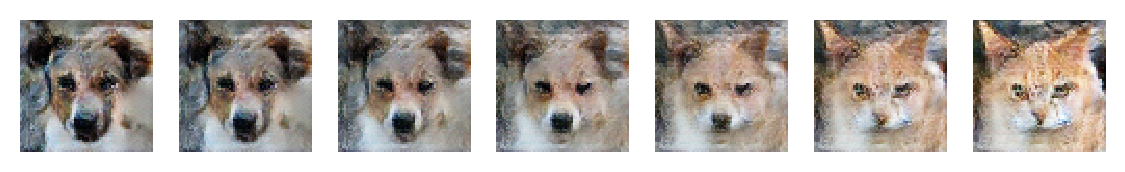
\includegraphics[width=15cm]{images/interpolation.png}
\caption{Generált képek lineáris interpolációval két zajvektor között}
\label{fig:interpolation}
\end{figure}

A bemeneti vektorok teréről feltételezhetjük, hogy folytonosan van kitöltve, mivel bármely pontra egy képet kaphatunk vissza. Viszont ezen tér feltérképezése sem egy triviális feladat, és az sem biztosított, hogy a talált pont környezetéből mintavételezve hasonló tulajdonságú képek generálhatóak ki.

A GAN tanítása során a Generátor a bemeneti vektorok terére megtanulja, hogy a tér egyes pontjaira milyen adatot képezzen le. A térből mintavételezett adatok mindegyikére egy, a tanítóhalmaz eloszlását követő adatot tud kigenerálni.
A tanítási lépések során általában normális vagy egyenletes eloszlás szerint generálunk pontokat, és azok alapján tanul a Generátor modellünk. Annak ellenére, hogy a tér egyes pontjaira igen jól betanul a modell, nem garantálható, hogy az így keletkezett tér megfelelően klaszterezhető lehet és valójában a tanítás során generált pontok eloszlását követik a klaszterek pontjai \cite{mukherjee2019clustergan}.

\Section{Képek közelítése pixel szinten}

A képek közelítésre egy megoldás lehet a \textit{synthesis-through-optimization} technika \cite{frans2021clipdraw}, amelyhez nem kell betanítani egy újabb modellt, csupán optimalizációs alapon történik meg a képek közelítése.
A technika megvalósításához szükségünk van egy olyan függvényre, amely adott bemenetre egy várt kimenetet generál, ez esetünkben a Generátor modell. Az bemenetre kapott kimenetet ezután meg kell vizsgálni, és egy célfüggvény segítségével ki kell értékelni, majd a hibaérték alapján módosítani kell a bemenetet olyan irányba, hogy a hiba csökkenjen.

A kimenet vizsgálatára általában egy osztályozót szokás alkalmazni. A következő alfejezetben ez a módszer kerül majd bemutatásra. Viszont a bemenet optimalizálási módszere egy egyszerűbb vizsgálati stratégia mellett kerül bemutatásra az egyszerűbben érthetőség kedvéért.

A GAN $G$ generátorának bemenete egy $\vec{z} \in \mathbb{R}^{z_n}$ vektor, ahol $z_n$ általában 100 szokott lenni. Vagyis a bemeneti vektor egy $z_n$ dimenziójú tér egy pontja. A 100 dimenzióban történő keresés igen nehéz lehet a hagyományos heurisztikus módszerekkel, mint például a hegymászó módszerrel. A hegymászó optimalizáló módszer során a célfüggvényt minimalizáljuk (vagy maximalizáljuk) a pont körüli tartomány mintavételezésével, majd a megfelelő szomszédos pontra való lépéssel. A bemeneti paraméter lehet a pont kiinduló pozíciója, a lépésköz és a mintavételezés sűrűsége. A megfelelő pontosság érdekében igen sok mintára lehet szükségünk, egy sokdimenziós térben pedig igen sok minta szükséges a tér feltérképezésére. A fix lépésköz és a mintavételezés pontatlanságának hatására könnyedén lokális optimumokban ragadhat az algoritmus. Több vizsgálandó pont elszórása a térben megnövelheti az esélyét annak, hogy rátalálunk a globális optimumra is, viszont ez jelentősen megnöveli a számításigényt.

A gradiens módszer vagy gradiens-süllyesztés (\textit{Gradient Descent}) egy olyan iteratív optimalizáló módszer, amely a differenciálható függvény lokális minimumának megtalására irányul. A célfüggvény elsőrendű deriváltjai igazítják el a vizsgált pontunkat a minimumhoz \cite{ruder2016overview}. A Gradiens módszer is fix lépésközökkel közelíti az optimumot, viszont ha a tér differenciálható, úgy a lépés iránya gyorsabban számolható, mint a hegymászó módszer esetében. Az optimalizálás tehát a Gradiens módszer segítségével kerül megvalósításra.

Két kép között a pixelszintű távolságot az L2 norma (vagy euklideszi norma) segítségével kaphatjuk meg, amely az
$$ \|x\|_2 = \left({\sum_{i=1}^{n}|x_i|^2}\right)^{\frac{1}{2}} $$
formában számítható.
Ezen távolságot L2- (vagy euklideszi) távolságnak is lehet nevezni. A kép egyes pixeleinek értékeit veszi csupán figyelembe. Az összehasonlításhoz a képeket ki kell nyújtani, hogy egy-egy vektort kapjunk.

Egy kiválasztott kép közelítése a bemeneti vektorok terében a következő módon történhet. Jelölje $X$ a keresendő képet, $G$ a generátort, $\vec{z} \in \mathbb{R}^{z_n}$ pedig a látens vektort.\\
A cél egy olyan $\vec{z} \in \mathbb{R}^{z_n}$ látens vektor keresése, amellyel a
$$ \sum_{i=1}^{n\times m}\sqrt{(X_i-G(\vec{z})_i)^2}$$
távolság minimalizálható.

A képeket tehát pixel szinten hasonlítjuk össze kiindulásképp.
Egyéb metrikákat is alkalmazhatunk a képek hasonlóságának mérésére, viszont az optimalizáló módszer bemutatásához ezen legegyszerűbb módszert választottam.

Legyen $l$ a lépésméret, $X \in \mathbb{R}^{n\times m \times 3}$ a keresendő kép, $G$ pedig a betanított Generátor. Jelöljük $t$-vel az időpillanatot.
\begin{enumerate}
	\item Generáljunk egy képet az aktuális $\vec{z}$ zajvektorral:
$$\hat X = G(\vec{z}).$$
	\item Számoljuk ki a generált kép és a keresendő kép távolságát:
$$ loss(\vec{z}) = \sum_{i=1}^{n\times m}\sqrt{(X_i-\hat X_i)^2}. $$
	\item Számoljuk ki a gradienseket a hibafüggvény szerint:
$$ grad(\vec{z}) = \frac{\mathrm{d}}{\mathrm{d}\vec{z}} \; loss(\vec{z}).$$
	\item Módosítsuk a $\vec{z}$ zajvektor elemeit a kapott gradiensek szerint egy $l$ hosszúságú lépéssel:
$$ \vec{z}^{\;(t)} = \vec{z}^{\;(t-1)} - l \cdot grad\left(\vec{z}^{\;(t-1)}\right).$$
	\item Ismételjük meg az algoritmust a konvergálásig.
\end{enumerate}

A kilépési feltétel nincs megadva, így az algoritmus előre meghatározott iterációszámig fut. A hibafüggvények változását esetleg nyomon követhetnénk, és ha két érték között oszcillál a hibafüggvény, akkor valószínűleg elért az algoritmus egy lokális minimumot. A példa egyszerűsítése kedvéért a lépésszám is egy bemeneti paraméter jelen esetben.

Az algoritmus Tensorflow-ban történő megvalósítása a következő:

\begin{python}
random_noise = tf.random.uniform([1, latent_dim], minval=-1, maxval=1)
noise = tf.Variable(random_noise)
step_size = 0.03
steps = 50
for i in range(steps):
    with tf.GradientTape() as g_tape:
        g_tape.watch(noise)
        generated_image = generator(noise, training=False)
        loss = tf.norm(goal_image - generated_image)
    gradients = g_tape.gradient(loss, noise)
    noise = noise - (step_size * gradients)
\end{python}

Az implementációban ügyelni kell arra, hogy a gradiensek meghatározásához szükséges változókon ne hajtsunk végre a TensorFlow-n kívüli módosításokat, hiszen olyankor a TensorFlow nem képes visszakövetni a gradiens számolást. Tehát ha például a számolás során mátrix műveleteket kell alkalmazunk a változóinkra, akkor azt egy külső csomag, például NumPy segítségével sajnos nem tehetjük meg. Viszont a TensorFlow-ban is megtalálhatóak a NumPy csomagból ismert eljárások, sokszor teljesen megegyező névvel és paraméterezéssel. Azért, hogy a bemeneti zajvektort módosítani lehessen, egy \texttt{tf.Variable} objektumot inicializálunk a zaj értékével. Ha ezt nem tennénk meg, a generált zaj konstans lenne, amelyet a módszer nem tudna megváltoztatni.

A Gradiens süllyesztés alapvető esetben fix lépésközökkel kerül végrehajtásra, viszont egy egyszerű bővítése lehet a módszernek a momentummal való kiegészítés. A momentum érték hatására a vizsgált pont nem csupán fix lépésekkel közlekedik a felületen, hanem a korábbi lépésköz figyelembe vételével változik az iterációkban elvégzett lépés távolsága.

Momentum esetén a változás a következőképpen kapható meg:
\begin{align*}
valtozas^{(t)} &= l \cdot \vec{grad} + momentum \cdot valtozas^{(t-1)}, \\
z_i^{(t)} &= z_i^{(t-1)} - valtozas^{(t)}.
\end{align*}

A momentum értékét 0 és 1 között szokás megadni. 0 momentum esetén valójában a momentum nélküli gradiens módszert kapjuk vissza.

Az alábbi kódrészletben egy olyan függvény található, amelyben a momentummal kiegészített gradiens módszer került implementálásra.
\begin{python}
def gradient_descent_momentum(goal_image, noise, step_size,
                              momentum, steps):
    change = 0
    for i in range(steps):
        with tf.GradientTape() as g_tape:
            g_tape.watch(noise)
            generated_image = generator(noise, training=False)
            loss = tf.norm(goal_image - generated_image)
        gradients = g_tape.gradient(loss, noise)
        change = (step_size * gradients) + momentum * change
        noise = noise - change
    return noise
\end{python}

A képek visszakeresésére $l=0.2$ lépésközzel és $0.9$ körüli momentum értékkel indítottam el az algoritmust. Ezen értékek megfelelőnek tűntek, viszont a paraméterek nagyban függnek a vizsgálandó Generátortól. A kép felbontásától, a látens dimenzió számától és a kiinduló zajtól is függ a paraméterek megválasztása.
A kiinduló zajt a pixelszintű visszakeresésnél az egyenletes eloszlásból generáltam ki a $[-1; 1]$ intervallumon. A bemeneti zajvektor eloszlása is egy olyan paraméter, amellyel érdemes kísérletezni.

\Aref{fig:gradlosses}. ábrán megfigyelhető a kétféle gradiens keresés során kapott hibaértékek változása, a kezdeti és a kiinduló zajvektor a keresés előtt és után, továbbá az ábra alján az egyes időpillanatokban kigenerált képek. Az ábrán megfigyelhető, hogy a momentum nélküli keresés során a konvergencia görbe sokkal simább, viszont hamar elér egy optimum pontot, amelyben megragad és nem képes ezután olyan nagy mértékben csökkenteni a hiba értéket. Ezzel szemben a momentummal történő keresés szemmel láthatóan átlépett ezen az optimumon a lendülete segítségével amikor a hibaértékei növekvő értékeket mutattak, majd egy olyan utat járt be, amely során jobban közelítette a keresendő zajvektort.

\begin{figure}[h]
\centering
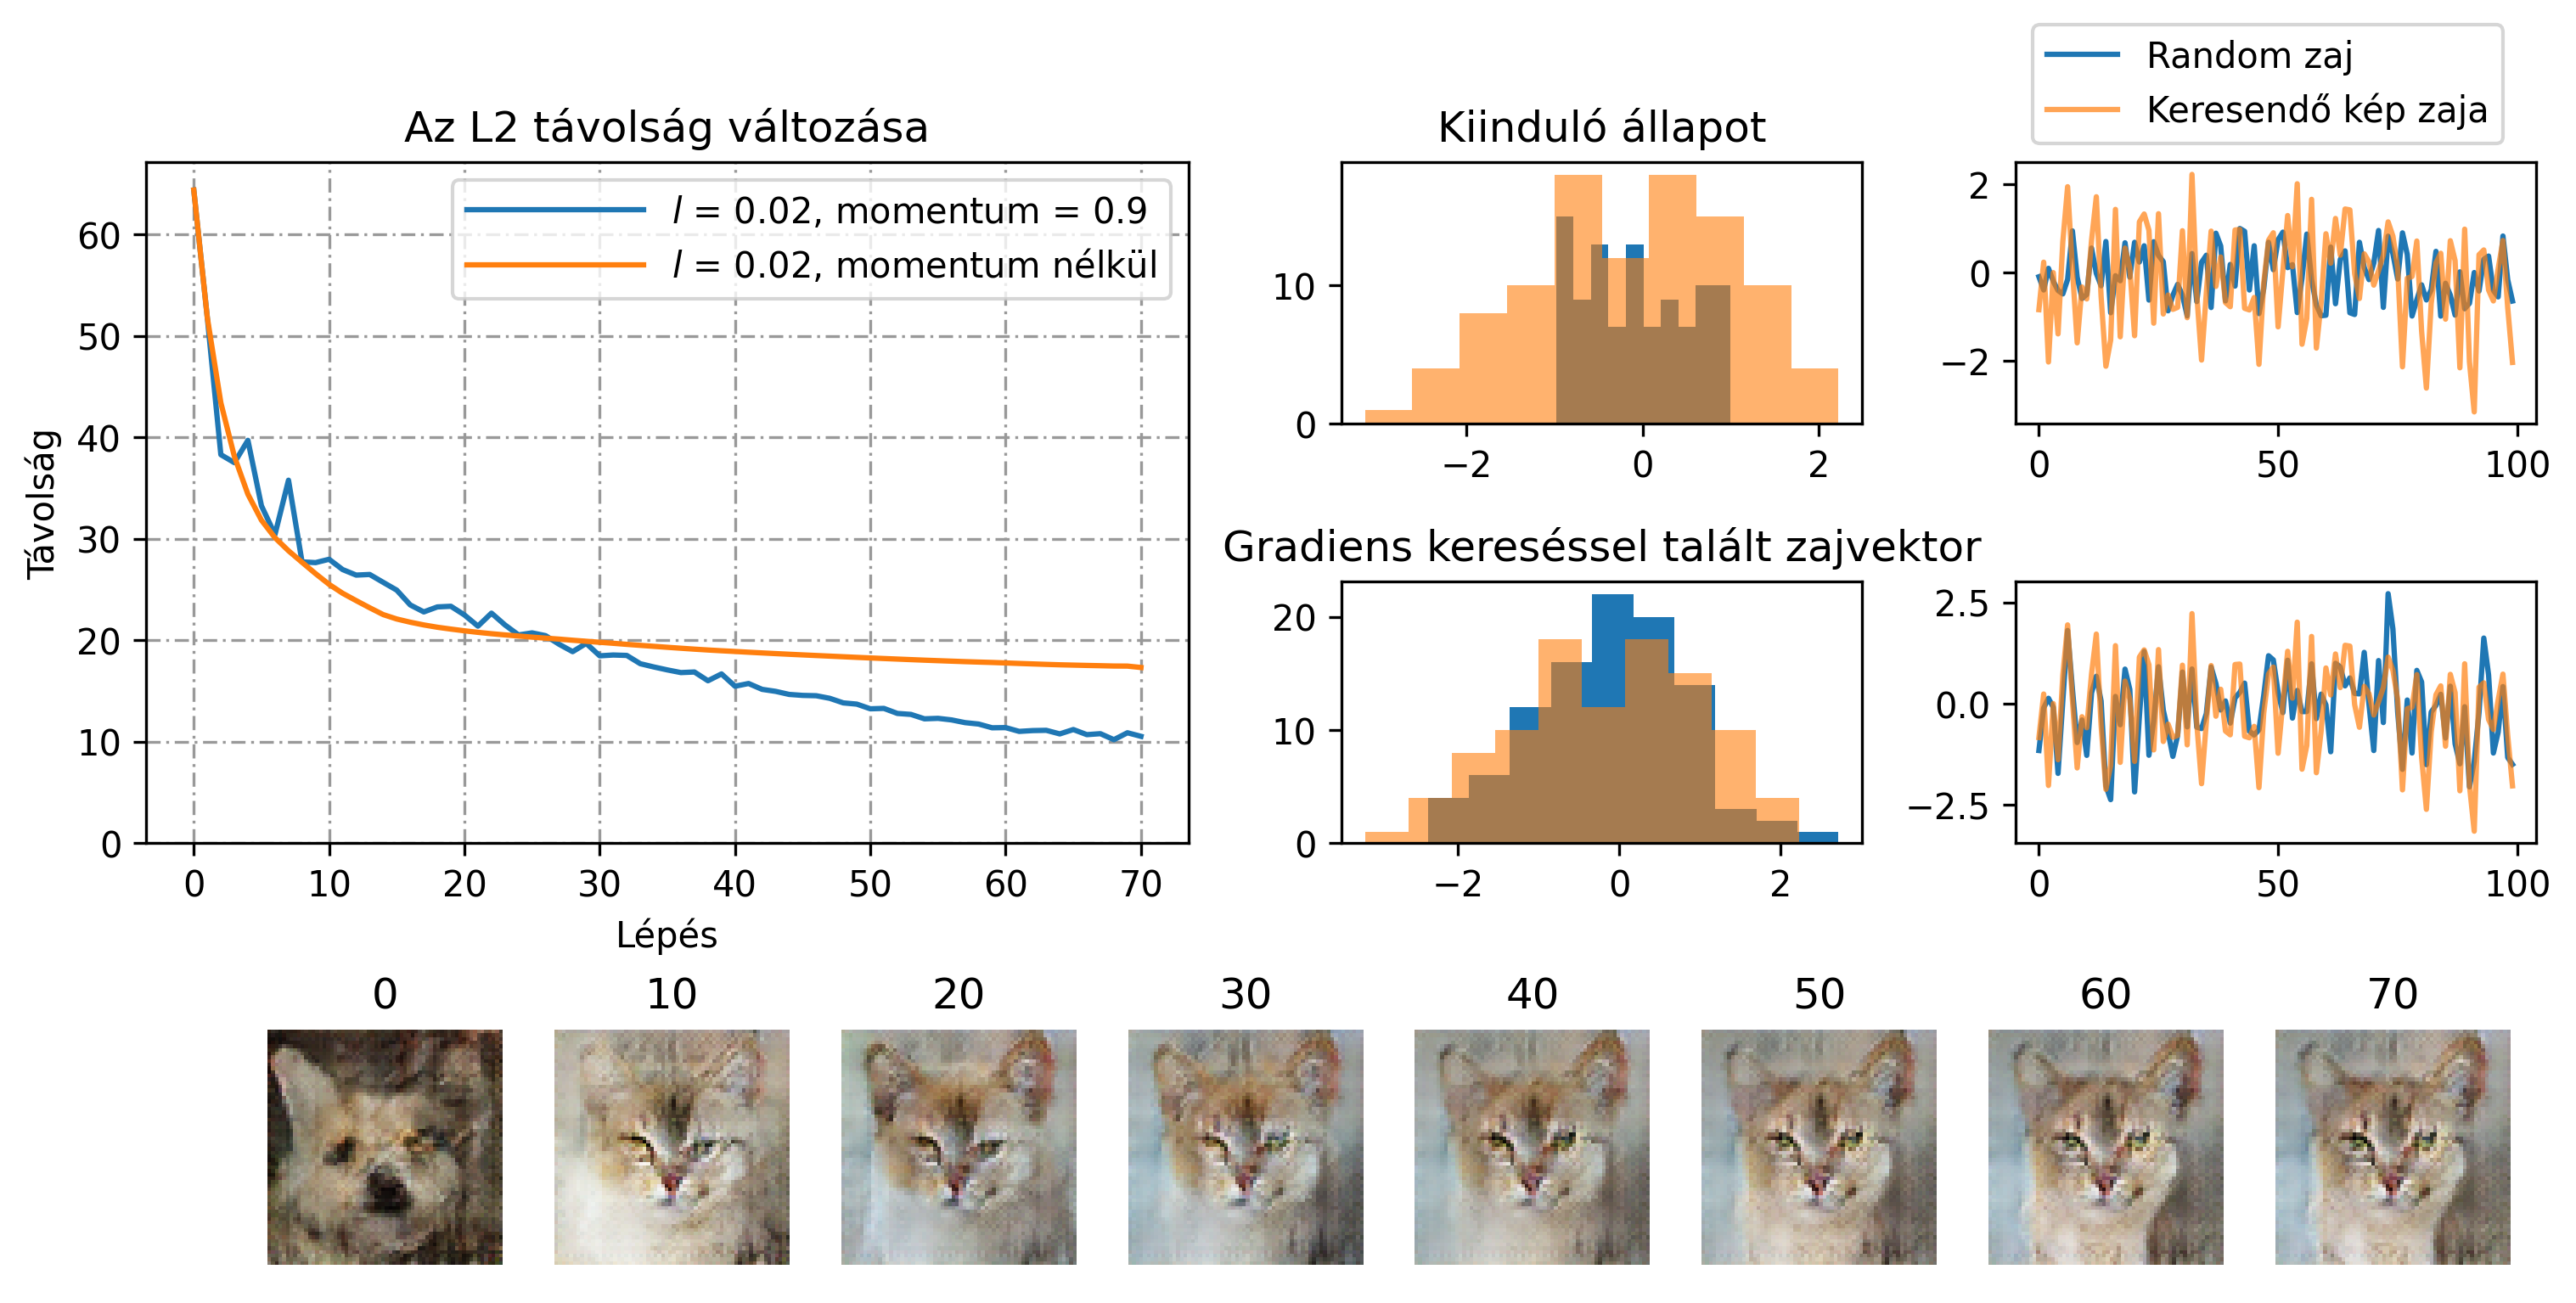
\includegraphics[width=15cm]{images/grad_losses.png}
\caption{A hibafüggvény változása a lépések során}
\label{fig:gradlosses}
\end{figure}

\Aref{fig:gradfound}. ábrán a keresendő zajvektorból generált kép, a kiinduló zaj képe és a momentum nélküli és a momentummal talált kimenet figyelhető meg. A momentummal történő keresés pontosabb találatot eredményezett, a momentum nélkül pedig igen közeli lokális optimum pontot kaptunk.

\begin{figure}[h]
\centering
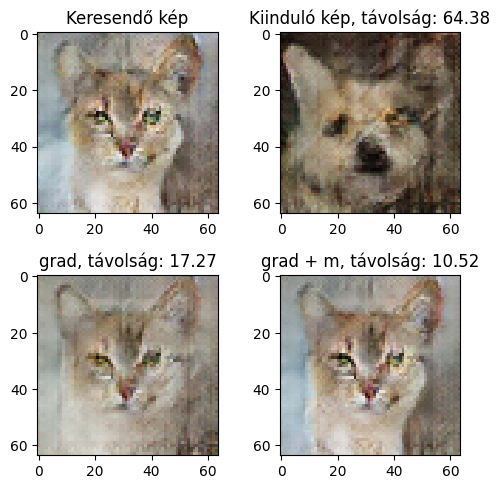
\includegraphics[width=8cm]{images/grad_found.png}
\caption{Gradiens kereséssel visszakeresett képek}
\label{fig:gradfound}
\end{figure}

\Aref{fig:gradval}. ábrán pedig egy, az adathalmaz validációs részéből kiválasztott képének visszakeresésének eredményét figyelhetjük meg. Ezen képet a GAN modell nem látta a tanulás során, viszont a kapott eredmény szemmel láthatóan egy corgi-t ábrázol, még ha nem is olyan kidolgozottan.

\begin{figure}[h]
	\centering
	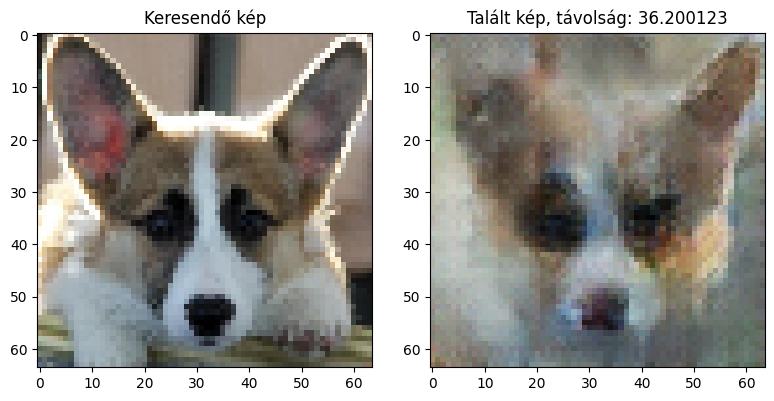
\includegraphics[width=8cm]{images/grad_search_val_image.png}
	\caption{A validációs halmaz egyik elemének visszakeresése}
	\label{fig:gradval}
\end{figure}


\Section{Képek keresése osztályozó segítségével}

A képek visszakeresése pixel szinten csupán azokban az esetekben adhat igazán jó megoldást, amikor a Generátor egy korábbi kimenetére végezzük el a keresést. Az előbbiekben erre láthattunk példát, \aref{fig:gradfound}. ábrán is az figyelhető meg, hogy a korábban kigenerált kép bemeneti vektorát hogyan sikerült a gradienslejtési módszerekkel (momentum nélkül és momentummal) visszakeresni.
Viszont ha egy külső forrásból érkező képet kívánunk így visszakeresni, akkor az eredményül kapott vektorból generált kép nem fogja olyan jól közelíteni a keresendő képet, hiába sikerült minimalizálnia a távolságot.
Ez értelemszerűen abból adódik, hogy az algoritmus a keresés során a nyers pixelértékeket veszi csupán csak figyelembe, a kép tartalmára tehát semmiféle információja nincsen. Viszont a Generátor nem képes minden pixelét egymástól függetlenül változtatni, hiszen a dekonvolúciós rétegeknek köszönhetően betanulta a tanítóhalmaz jellegzetességeit, és a kigenerált képek is a tanítóhalmaz eloszlását követik. Így nem létezhet olyan bemeneti vektor, amellyel tetszőleges pixelértékeket felvehet a kimeneti kép.

Ha az eredeti adathalmazból  kívánunk képeket visszakeresni, akkor közelítő eredményeket kaphatunk (mint ahogyan az \aref{fig:gradval}. ábrán is látszik), viszont ezek továbbra sem lesznek tökéletes találtatok, hiszen a GAN nem pixel pontosan tanulja be az adathalmaz elemeit, hanem azok jellegzetességeit tanulja meg reprezentálni, ezért is nevezik a GAN-t \textit{Representation-learning} \cite{geron2019hands} modellnek is.

Ha a hibafüggvényt kicseréljük, és az optimalizációt egy, az adathalmazon tanított osztályozóval végezzük el, úgy viszonylag jó találatot kaphatunk. Természetesen ilyenkor az osztályozó teljesítményétől is függ az eredmény jósága.

Az irodalomkutatás során egyetlen munkát találtam, amely publikálva is volt (CLIP\-DRAW \cite{frans2021clipdraw}), amely ilyen megoldást használ. A további ismertebb munkák csupán notebook-ok formájában érhetőek el. Viszont a közös bennük, hogy mind a CLIP \cite{radford2021learning} osztályozó kimenetei alapján végzik el az optimalizációt.

Egy hasonló megoldást alkalmaztam, viszont a CLIP osztályozó helyett egy saját modellt tanítottam be. A betanított osztályozó modell alapja az Inception v3, amely a témám során több helyen is feltűnt, az IS és FID pontok számítása is ezen modellen alapszik. Az ImageNet \cite{deng2009imagenet} adatbázison tanított Inception modell az adatbázis 1000 darab osztályára képes osztályozni. Ha a modellt használni kívánjuk a saját osztályozónkba, akkor az úgynevezett \textit{Transfer-learning} \cite{tensorflow} technikát kell alkalmazni a tanításhoz, amelynek lényege, hogy egy, már betanított általános modellre egy újabb modellt építünk, amely egy szűkebb, speciális feladat megoldására szánunk. Esetünkben nincs szükség 1000 darab osztályra. Az Inception modellt felhasználhatjuk a képek jellegeinek kinyerésére, és a modell utolsó rétegét pedig kicseréljük a saját osztályozónkra. A kapott modell tanítása egyszerűbbé válik, mintha az alapoktól kellene egy új modellt betanítanunk.

A tanítás során az eredeti modell súlyait "lefagyasztjuk", vagyis a háló ezen részének paramétereit taníthatatlanná tesszük, és a tanítás során csak az általunk hozzáadott rétegeket frissítjük.
A hibafüggvény számoláshoz a Kategórikus Kereszt-entrópiát (\textit{Categorical Cross-Entropy}) használjuk fel. Az osztályozó modell tanítása ezek után a teljesen megszokott módon történik.

Az alábbi kódrészletben az osztályozó modell implementációja figyelhető meg.
\begin{python}
inputs = keras.Input(shape=(64, 64, 3))
x = data_augmentation(inputs)
resized = tf.image.resize(
    x, [299, 299],
    preserve_aspect_ratio=True, method='nearest'
)
x = inception_model(resized, training=False)
x = keras.layers.GlobalAveragePooling2D()(x)
x = keras.layers.Dropout(0.2)(x)
x = keras.layers.Dense(3)(x)
outputs = keras.layers.Activation("softmax")(x)
model = keras.Model(inputs, outputs)
\end{python}

Az újonnan kialakított modell bemenete megegyezik a betanított Generátor kimenetével. Az \textit{overfitting} elkerülése érdekében, és hogy a modell ne az egyes, számára érdekes pixelértékek alapján hozza meg a döntést, a bemenetre \textit{data augmentation} technika kerül alkalmazásra, amely véletlenszerű minimális transzformációkat alkalmaz a képekre. A bemeneti képeket véletlenszerűen függőlegesen tükrözi, és szintén véletlenszerűen elforgatja. A Cifar-10 adathalmaz esetében azt figyeltem meg, hogy az augmentation technika csak megnehezíti a konvergenciát, és a modell nagyon sokat tévedett ennek hatására. A technika kihagyásával a tanítás jobb eredményt hozott, viszont ezen adathalmaz sokkal több tanítómintával rendelkezik, mint az AFHQ és a benne található képek is változatosabbak, így esetében lehetséges, hogy valóban nem indokolt a technika használata.

Az \texttt{inception\_model} a kódrészletben a már említett, csonkított változata az eredetinek. Az utolsó \texttt{Dense} rétegétől megfosztott változata, a lefagyasztott súlyokkal. Az Inception modell bemenetként $299 \times 299$ felbontású képet vár, így a képünket fel kell nagyítani a kívánt felbontásra. A nagyításhoz \textit{nearest} interpolációt alkalmaztam, hogy a felbontás növelése ne járjon homályossággal, ugyanis azt figyeltem meg, hogy olyankor a modell gyengébben teljesít.

A csonkított Inception modell kimenete egy $(8, 8, 2048)$ alakú tenzor, amely a bemeneti képekből kinyert feature-öket tartalmazza. A \texttt{GlobalAveragePooling2D} réteg az előbbi kimenetből 2048 elemű vektort készít, amelyet beadhatunk az utolsó \texttt{Dense} rétegnek, amely az osztályozást végzi el. Egy regularizációs technikaként, hogy csökkentsük az overfitting esélyét, egy \texttt{Dropout} réteg is helyet kapott a teljesen összekapcsolt réteg előtt.
A kimenetet \texttt{softmax} aktivációs függvénnyel normalizáljuk, így a modell használata során kimenetként megkapjuk az egyes osztályokhoz tartozó valószínűségi értékeket.

A kapott modellnek összesen 21 808 931 darab paramétere van, melyből csupán 6147 a tanítható. A tanítás során tehát az osztályozásért felelős rétegeket kell csupán frissítenünk.

Az optimalizálást a GAN tanításánál is használt Adam optimalizálóval végeztem, 0.0001 \textit{learning-rate} paraméterrel. A bemeneti dataset-et 32 elemű mini-batch-ekre osztottam fel. A tanítást mindösszesen 10 epoch-ig futtattam. A nagy tanítóminta és a kevés tanítható paraméter miatt azt figyeltem meg, hogy elegendő ennyi tanítás is. A konvergenciagörbe a Cifar-10 dataset-re tanítva \aref{fig:transfer_learning_loss}. ábrán látható, az osztályozás eredményeit bemutató confusion mátrix pedig \aref{fig:transfer_confusion}. ábrán.

\begin{figure}[h]
	\centering
	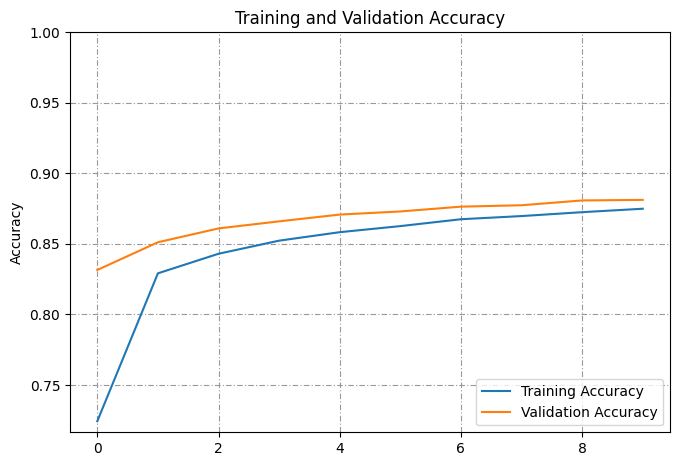
\includegraphics[width=10cm]{images/transfer_inception.png}
	\caption{Transfer-learning loss értékek (Inception modell alapú)}
	\label{fig:transfer_learning_loss}
\end{figure}

\begin{figure}[h]
	\centering
	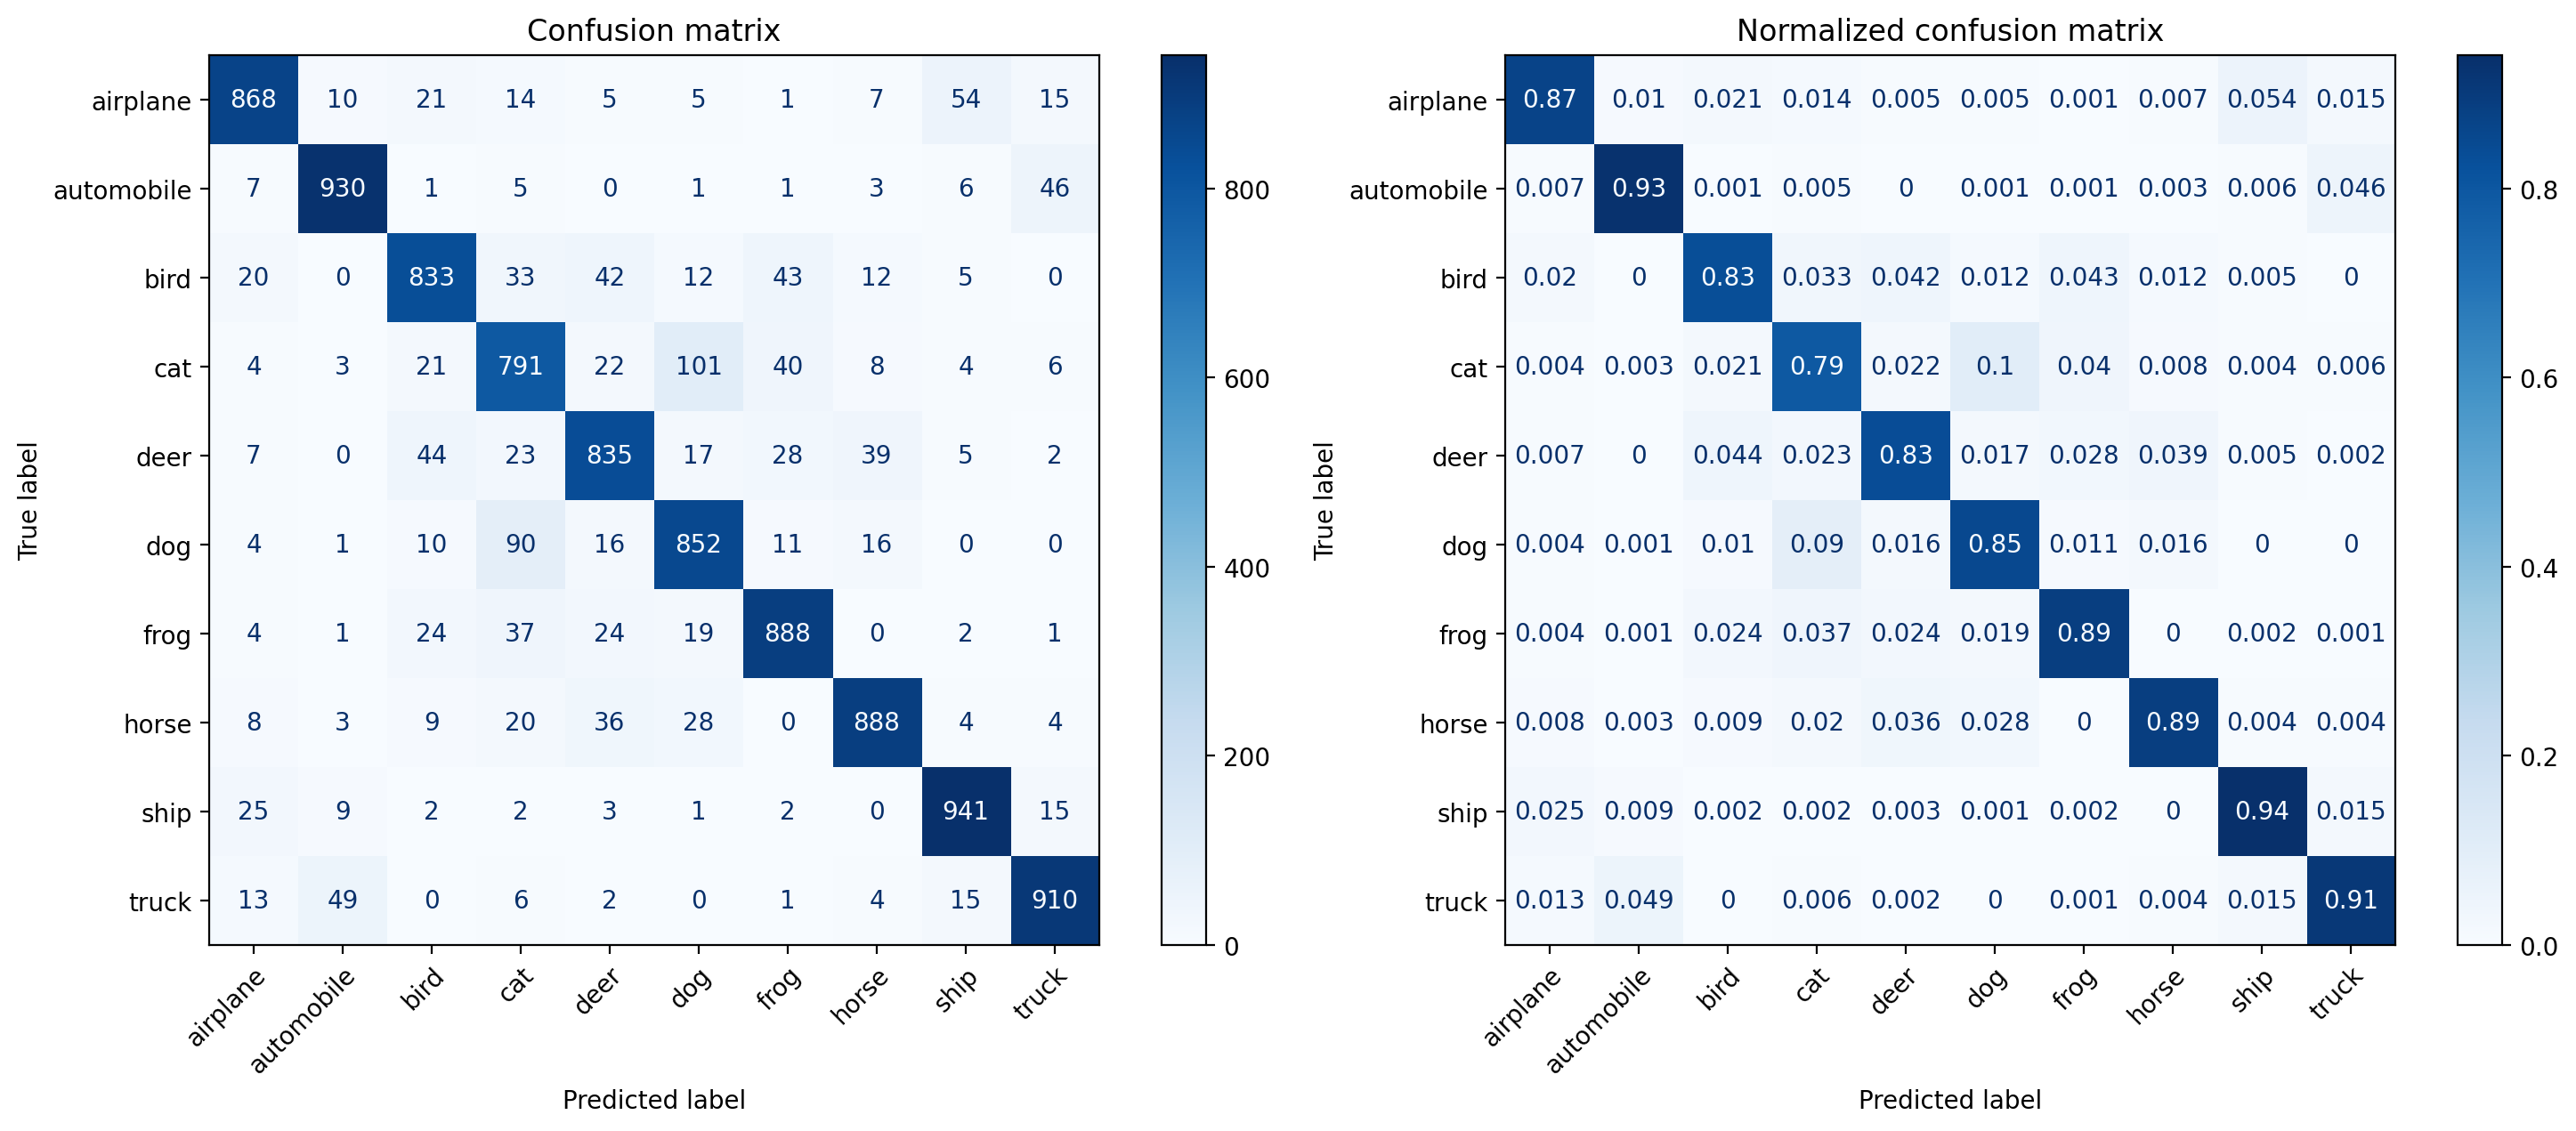
\includegraphics[width=15cm]{images/transfer_confusion.png}
	\caption{Confusion mátrix (Inception modell alapú)}
	\label{fig:transfer_confusion}
\end{figure}

Mivel a GAN tanítása után a Diszkriminátort elhagyjuk, és további szerepe nincsen, úgy gondoltam, hogy akár hasonló módon is felhasználásra kerülhet, mint az előbbiekben ismertetett Inception modell. A tanulás során természetesen nem csupán a tanítóhalmazt látta a Diszkriminátor, hanem a generált képeket is, így elég specifikus tudással rendelkezik csupán. A háló súlyai úgy lettek optimalizálva, hogy belső reprezentációt állítson elő, amellyel a bináris osztályozást megfelelően el tudja végezni. Így a háló által kinyert jellegvektorok is oly módon állnak össze, hogy el tudja az alapján dönteni, hogy a kép valódi vagy hamis. A tanítást elvégeztem, viszont az így kapott összeállított új modell teljesítménye alulmaradt az Inception-t használó másik modellel szemben. A konvergencia görbe \aref{fig:transfer_learning_loss_discriminator}. ábrán figyelhető meg, a confusion mátrix pedig \aref{fig:transfer_confusion_disc}. ábrán látható.

\begin{figure}[h!]
	\centering
	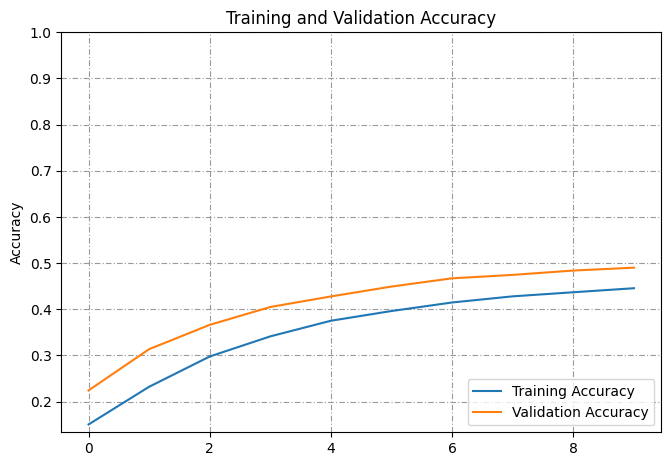
\includegraphics[width=10cm]{images/transfer_discriminator.png}
	\caption{Transfer-learning loss ábra (Diszkriminátor modell alapú)}
	\label{fig:transfer_learning_loss_discriminator}
\end{figure}

\begin{figure}[h!]
	\centering
	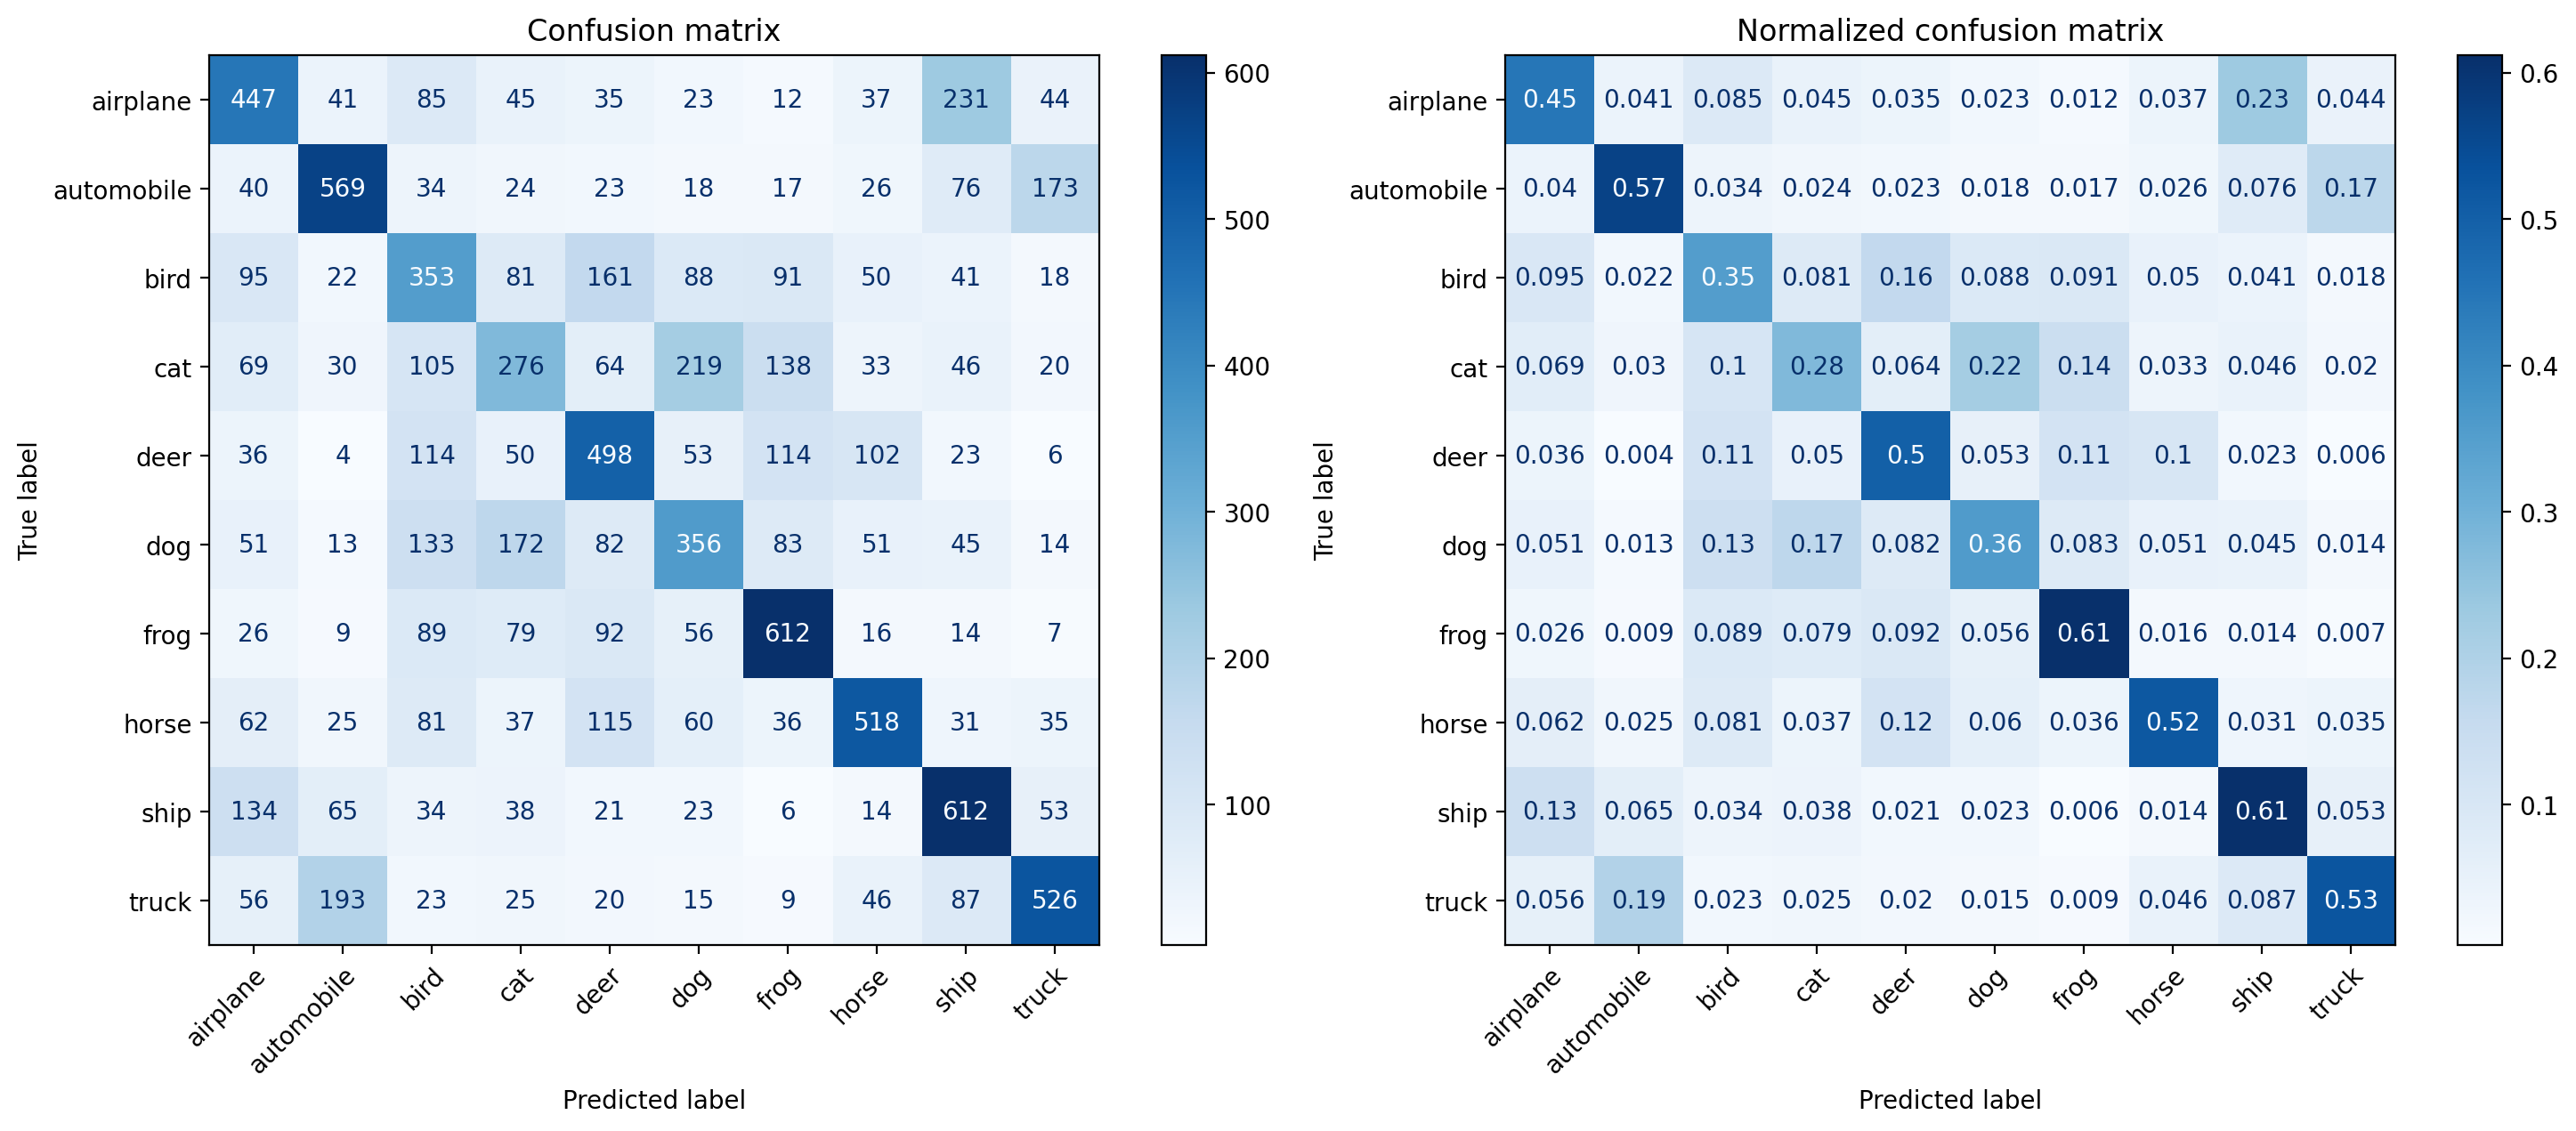
\includegraphics[width=15cm]{images/transfer_discriminator_confusion.png}
	\caption{Confusion mátrix (Diszkriminátor modell alapú)}
	\label{fig:transfer_confusion_disc}
\end{figure}


A bemeneti vektorok visszakeresése pedig a már ismertetett gradiens süllyesztés módszerrel valósul meg, viszont a hibafüggvény számolása a Kategórikus Kereszt-entrópia által kerül meghatározásra, hasonlóan, mint az osztályozó tanításánál. Az algoritmus bemenete tehát a kezdeti zajvektor, a keresendő címke és a gradiens módszer paraméterei (a lépésköz, a momentum és az iterációszám).
A bemeneti címkét \textit{One-Hot} enkódolással kell megadni a keresztentrópia számoláshoz, ugyanis az új osztályozó modell kimenete az adott osztályok valószínűségi értékei lesznek. A gradiens kereséssel pedig a keresztentrópia értéket kívánjuk csökkenteni. Tehát ha egy adott osztályra kívánunk egy olyan vektort kapni, amelyből a megfelelő osztályba tartozó képet ki tudja generálni a Generátor, akkor ebben az esetben az osztályhoz tartozó valószínűségi érték 1 lesz, a többi osztályé pedig 0.

Amennyiben kevert osztályra kívánunk képet generálni, úgy olyan keresendő one-hot enkódolást kell megadnunk, amelyben a kívánt osztályok megfelelő súlyokkal rendelkeznek. Mivel a GAN tere folytonosan van kitöltve, így feltehető, hogy létezik olyan pont a térben, amely egyszerre több osztály jellegzetességeit is magában hordozza. A \ref{fig:interpolation} ábrán is megfigyelhető, hogy az interpoláció mintavételezett pontjaiban a két végpont között milyen folytonos az átmenet és a köztes állapotokban mindkét pont tulajdonságai megjelennek.

Az eljárás optimális paraméterei ebben az esetben is több tényezőtől függnek. Az osztályozó modell teljesítménye, az osztályok száma is igen nagy befolyásoló tényező lehet a megfelelő lépésköz és momentum kiválasztására.  Megfigyeléseim szerint a megfelelő eredmények elérése érdekében a lépésközt a pixelszintű kereséstől is alacsonyabbra érdemes választani, például $l=0.005$ lépésközzel és $0.09$-es momentum értékkel az AFHQ adathalmazon tanult modellekkel értékelhető találatokat kaphatunk. A túl magas lépésköz hatására a keresés során a látens tér olyan területeire is tévedhet az algoritmus, amelyre a generátor szaturált képeket tud előállítani csupán.

\Aref{fig:searching}. és \aref{fig:searching_ship}. ábrákon láthatunk példát a macska, illetve hajó címkével történő keresésre.

A \ref{fig:collapsed_mode} ábrán is szemléltetett, a generátorban kialakuló összeomlott-mode-ok a keresési folyamat során is bosszúságot okozhatnak. Amint belépünk egy ilyen területre a keresés során, az algoritmus nem képes kilépni, hiszen az osztályozó egyszerre látja mindegyik osztály jellegzetességeit a vizsgált képen.

\begin{figure}[h]
	\centering
	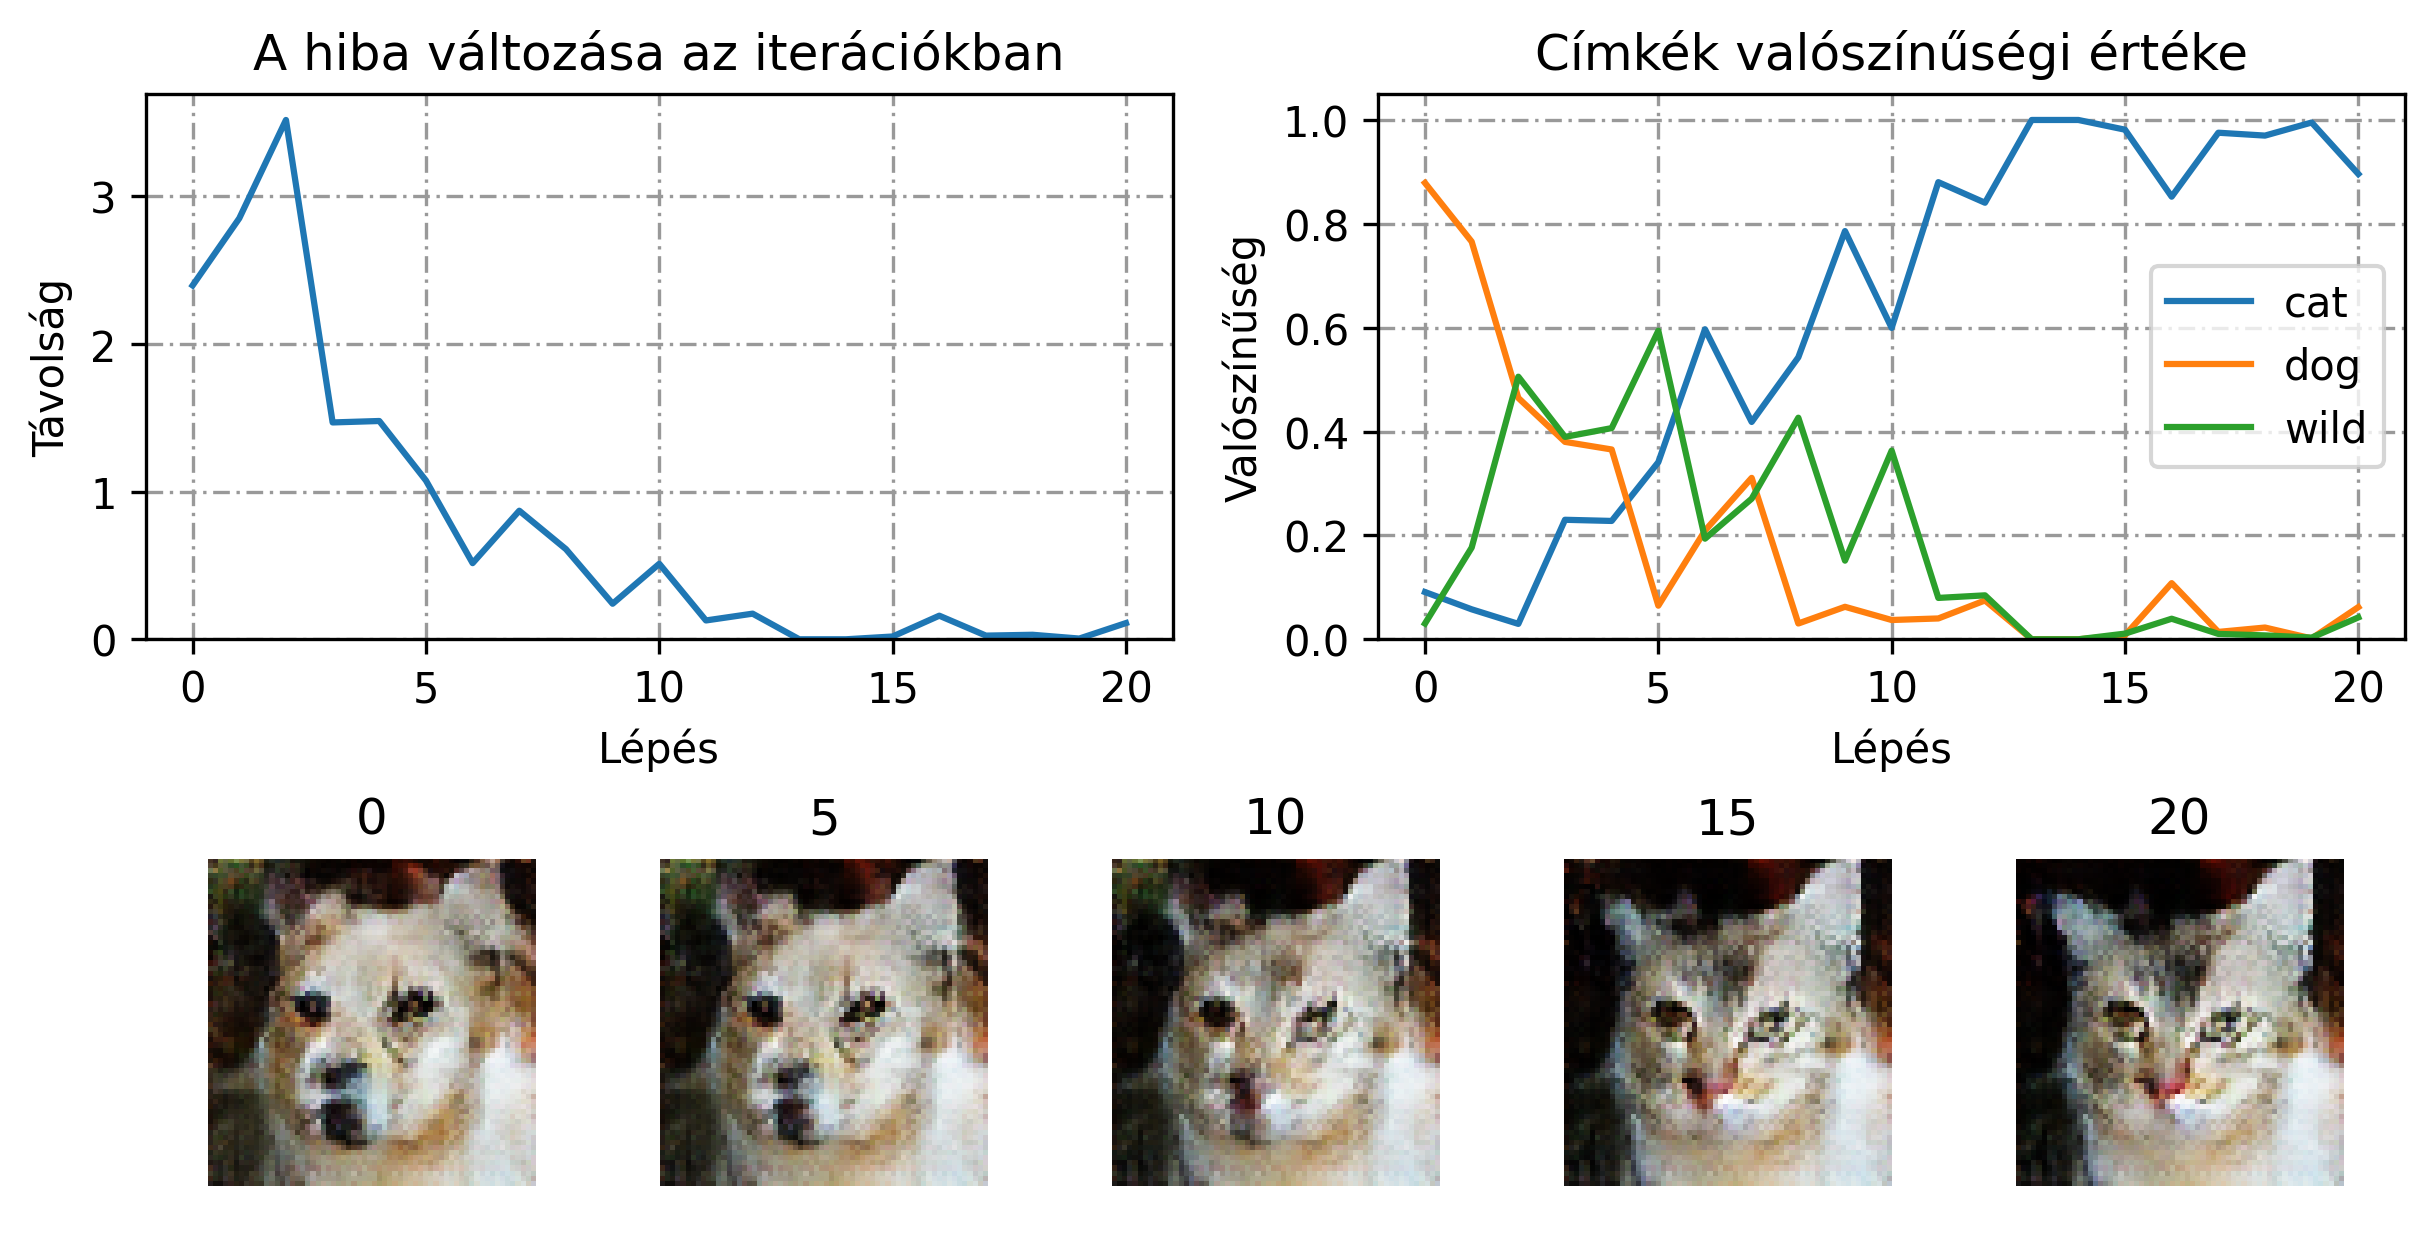
\includegraphics[width=\textwidth]{images/searching-cat.png}
	\caption{Kép generálása osztály szerint (Macska címkével)}
	\label{fig:searching}
\end{figure}

\begin{figure}[h]
	\centering
	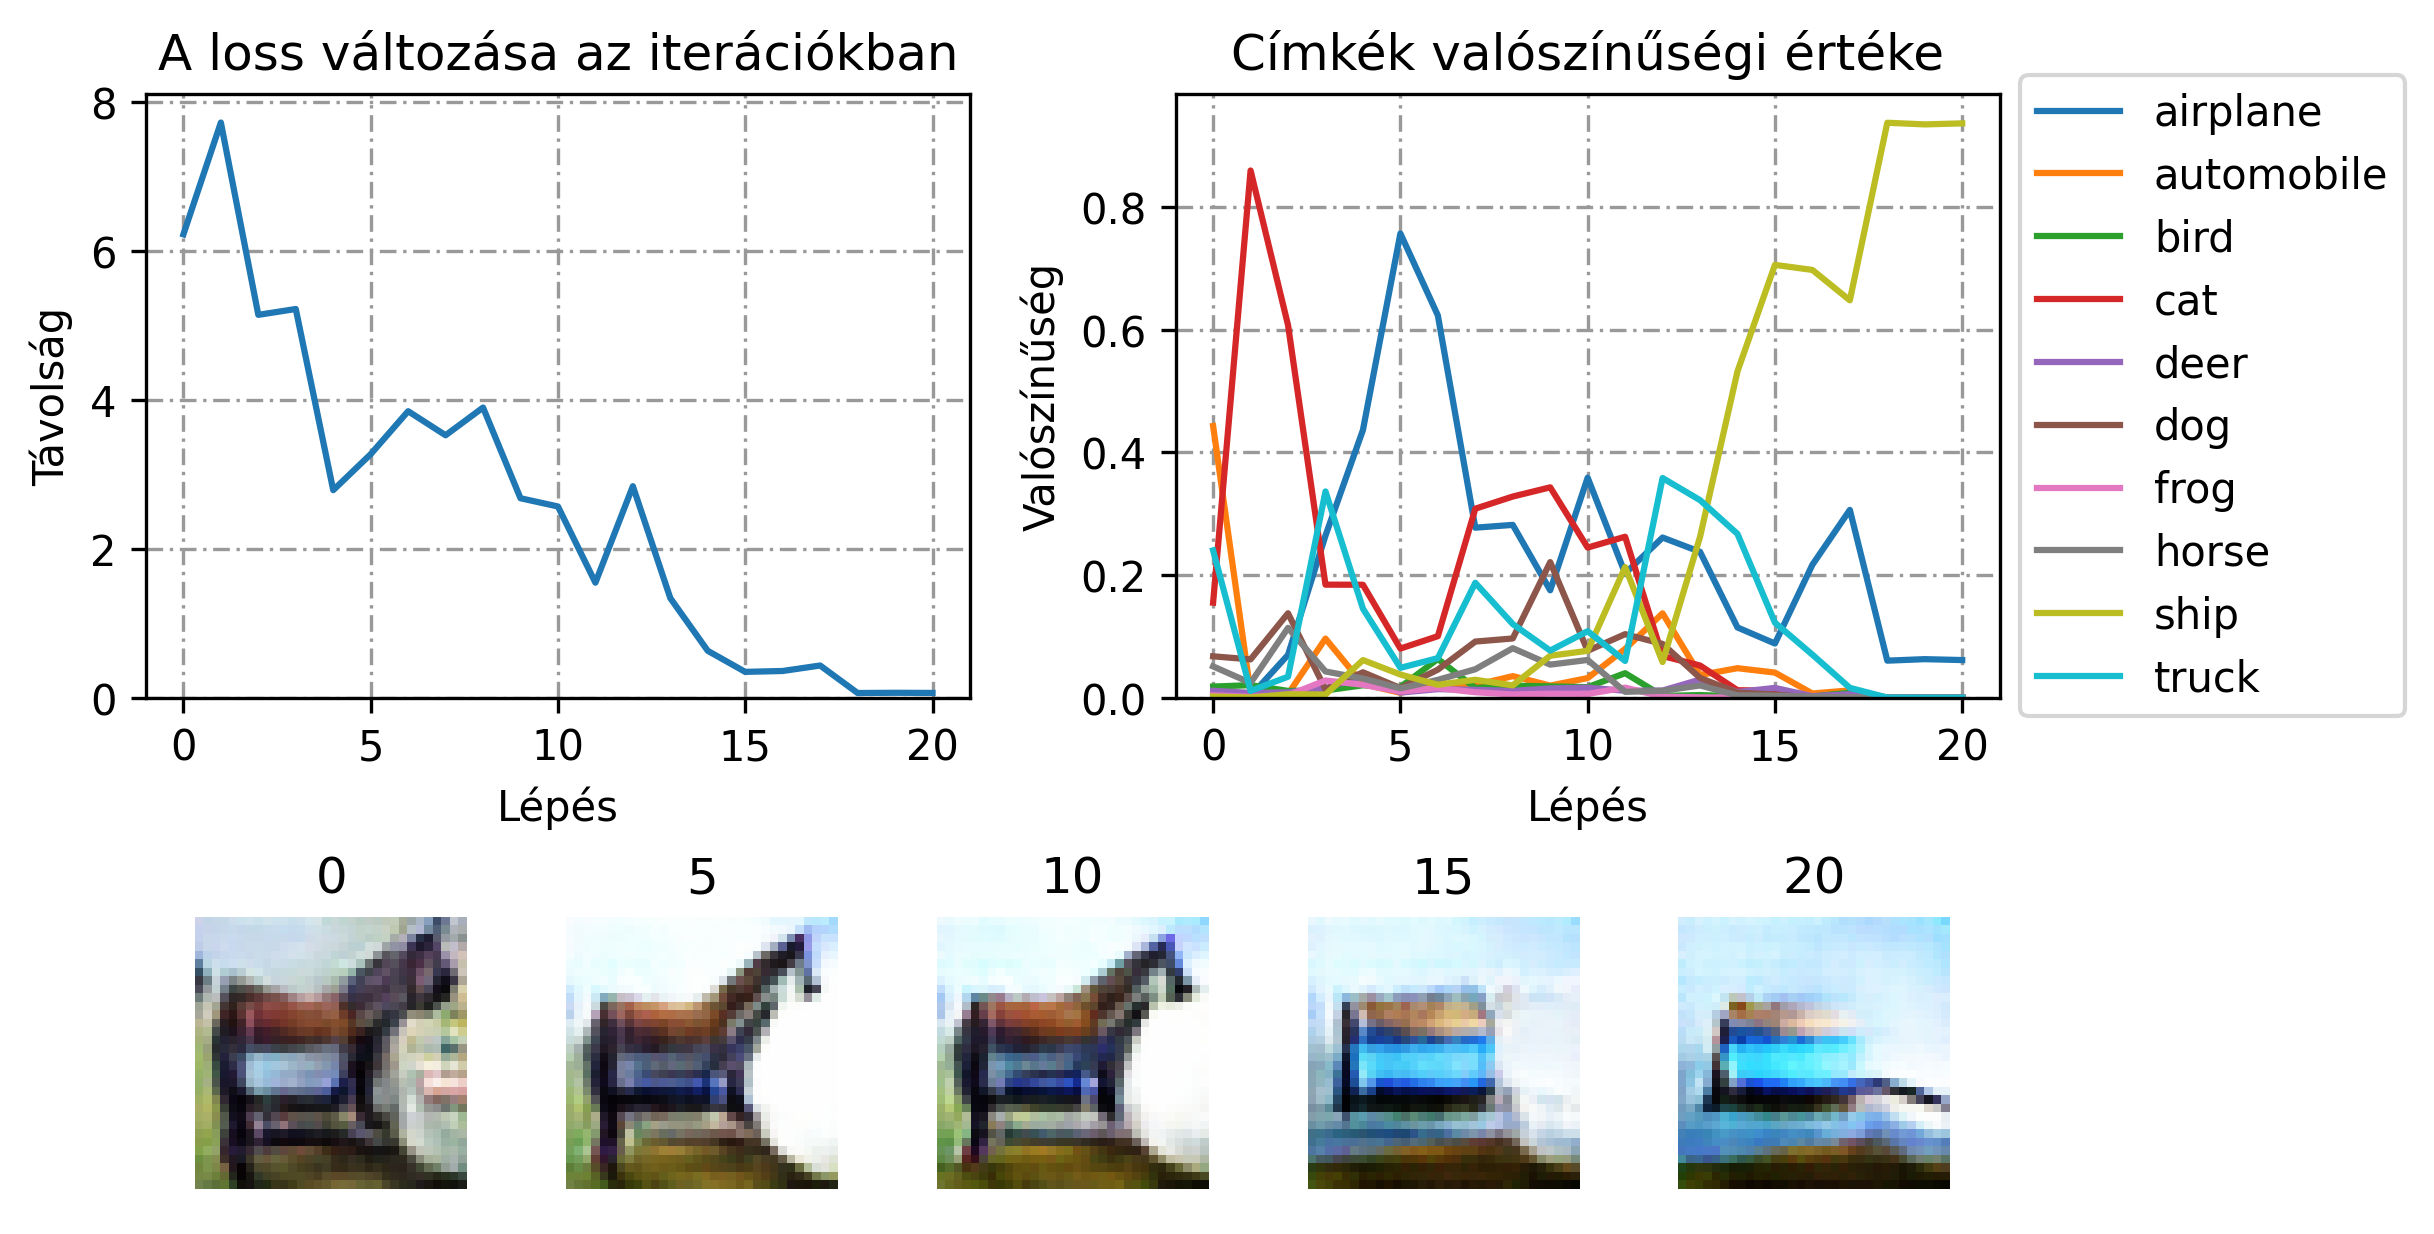
\includegraphics[width=\textwidth]{images/searching-cifar_ship.png}
	\caption{Kép generálása osztály szerint (Hajó címkével)}
	\label{fig:searching_ship}
\end{figure}
